% ============================================================
%  Semana 7 · Clase 14: Dashboard e identificación de insights
%  Curso: Análisis y Visualización de Datos para la Toma de Decisiones
%
%  Formato de la sesión (3 h), en forma de guía paso a paso:
%    Hora 1. Del modelo al tablero: preparar el modelo, tarjetas, barras,
%            columnas y formato
%    Hora 2. Tiempo, anomalías, relación y lugar: líneas, tendencia,
%            anomalías, dispersión y mapas
%    Hora 3. Del gráfico al insight: validación de cifras, coherencia
%            entre objetos visuales y ficha de insights
%
%  Datos: datos/gimnasio_vitalis.xlsx (el mismo archivo de la Clase 13,
%  generado con ../../../scripts/semana07-clase13_datos.py)
%
%  Las capturas de figuras/ms-learn/ provienen de Microsoft Learn y se
%  usan sin modificar, según la política de Microsoft para capturas de
%  pantalla de sus productos ("Used with permission from Microsoft").
%
%  Compilar (dos veces) directamente desde esta carpeta:
%    xelatex semana07-clase14.tex
%    xelatex semana07-clase14.tex
% ============================================================
\documentclass[aspectratio=169,11pt]{beamer}

\usepackage{../../../plantilla/beamerthemeesumer}
\usetheme{esumer}

\usepackage[spanish,es-noshorthands]{babel}
\usepackage{booktabs}
\usepackage{graphicx}
\usepackage{array}
\newcolumntype{L}[1]{>{\raggedright\arraybackslash}p{#1}}
\usetikzlibrary{arrows.meta,positioning,calc}

% ---------------- DATOS DE LA CLASE ----------------
\title{Dashboard e identificación de insights}
\subtitle{Guía paso a paso con los datos del Gimnasio Vitalis}
\author{Docente: Cristian A. Jimenez C., MSc}
\date{Oct 20 al 25}

\setmodulo{Módulo 3: Experimentar (Visualización e Insights)}
\setsemana{7}
\setclase{14}
\setfechaclase{Oct 20 al 25}
\setmodalidad{Virtual}
% -----------------------------------------------------

\graphicspath{{figuras/}}

% Pie de cada captura: producto, página de origen y la frase que exige Microsoft
\newcommand{\fuente}[2]{%
  \par\vspace{1pt}{\fontsize{5.5}{6.5}\selectfont\color{black!55}%
  Captura de Microsoft Power BI Desktop. Guía oficial de este paso:
  \href{#2}{\color{esumerOrange}«#1»}. Used with permission from Microsoft.\par}}

% Pie para los pasos sin captura: solo el enlace a la guía oficial
\newcommand{\guia}[2]{%
  \par\vspace{1pt}{\fontsize{6}{7}\selectfont\color{black!55}%
  Guía oficial de este paso: \href{#2}{\color{esumerOrange}«#1»}.\par}}

% Número de paso
\newcommand{\npaso}[1]{\tikz[baseline=(n.base)]\node[circle,fill=esumerOrange,
  text=white,font=\bfseries\footnotesize,inner sep=0pt,minimum size=0.48cm](n){#1};}

% Fórmula DAX en un recuadro sin título
\newcommand{\codigo}[1]{\par\smallskip\noindent\colorbox{esumerGray!70}{\parbox{\dimexpr\linewidth-2\fboxsep\relax}{\scriptsize\ttfamily #1}}\par\smallskip}

% Menú de Power BI: nombre en español (nombre en inglés)
\newcommand{\menu}[2]{\textbf{#1} {\color{black!55}(#2)}}

\newcommand{\urlinstalar}{https://learn.microsoft.com/es-es/power-bi/fundamentals/desktop-get-the-desktop}
\newcommand{\urlstore}{https://apps.microsoft.com/detail/9ntxr16hnw1t?hl=es-co}
\newcommand{\urlcentro}{https://www.microsoft.com/download/details.aspx?id=58494}
\newcommand{\urldatos}{https://github.com/craljimenez/An-lisis_y_Visualizacion_de_Datos_para_la_Toma_de_Decisiones/raw/main/clases/semana07-clase14-dashboard-identificacion-insights/datos/gimnasio_vitalis.xlsx}
\newcommand{\urlinforme}{https://learn.microsoft.com/es-es/power-bi/create-reports/desktop-report-view}
\newcommand{\urlagregar}{https://learn.microsoft.com/es-es/power-bi/visuals/power-bi-report-add-visualizations-i}
\newcommand{\urltarjeta}{https://learn.microsoft.com/es-es/power-bi/visuals/power-bi-visualization-card}
\newcommand{\urlformato}{https://learn.microsoft.com/es-es/power-bi/visuals/service-getting-started-with-color-formatting-and-axis-properties}
\newcommand{\urlcolumnas}{https://learn.microsoft.com/es-es/power-bi/visuals/power-bi-visualization-column-charts}
\newcommand{\urllineas}{https://learn.microsoft.com/es-es/power-bi/visuals/power-bi-line-chart}
\newcommand{\urlanalisis}{https://learn.microsoft.com/es-es/power-bi/transform-model/desktop-analytics-pane}
\newcommand{\urlanomalias}{https://learn.microsoft.com/es-es/power-bi/visuals/power-bi-visualization-anomaly-detection}
\newcommand{\urlfiltros}{https://learn.microsoft.com/es-es/power-bi/create-reports/power-bi-report-add-filter}
\newcommand{\urldispersion}{https://learn.microsoft.com/es-es/power-bi/visuals/power-bi-visualization-scatter}
\newcommand{\urlazuremaps}{https://learn.microsoft.com/es-es/azure/azure-maps/power-bi-visual-get-started}
\newcommand{\urlcoropletico}{https://learn.microsoft.com/es-es/power-bi/visuals/power-bi-visualization-filled-maps-choropleths}
\newcommand{\urlcategoria}{https://learn.microsoft.com/es-es/power-bi/transform-model/desktop-data-categorization}
\newcommand{\urltipos}{https://learn.microsoft.com/es-es/power-bi/visuals/power-bi-visualization-types-for-reports-and-q-and-a}

\begin{document}

{
\setbeamertemplate{footline}{}
\begin{frame}[plain,noframenumbering]
  \titlepage
\end{frame}
}

\begin{frame}[t]{Agenda de hoy (3 horas)}
  \begin{columns}[T,onlytextwidth]
    \column{0.32\textwidth}
    \begin{block}{Hora 1}
      \small Del modelo al tablero: preparar el modelo y crear tarjetas,
      barras y columnas con buen formato.
    \end{block}
    \column{0.32\textwidth}
    \begin{block}{Hora 2}
      \small Tiempo, relación y lugar: líneas, tendencia, una anomalía,
      dispersión y cuatro usos de los mapas.
    \end{block}
    \column{0.32\textwidth}
    \begin{block}{Hora 3}
      \small Del gráfico al insight: validar cifras, revisar la coherencia
      y escribir una ficha de 3 a 5 insights.
    \end{block}
  \end{columns}
  \vspace{0.3cm}
  \small En la Clase 13 construiste el modelo. Hoy le haces preguntas con
  gráficos y conviertes las respuestas en \textbf{recomendaciones} que
  alguien pueda usar para decidir.
\end{frame}

\begin{frame}[t]{Cómo leer esta guía}
  \small
  Es la misma forma de la Clase 13: una \textbf{guía para seguir con Power
  BI abierto}.
  \vspace{0.1cm}
  \begin{itemize}
    \small
    \item \npaso{4}\; \textbf{Un número naranja}: algo que haces tú, en
      orden. Cada paso usa lo que hiciste en los anteriores.
    \item \textbf{Captura oficial} de Microsoft y, al lado, las
      instrucciones. Los menús aparecen como \menu{Nombre en
      español}{nombre en inglés}.
    \item Debajo, en naranja, el \textbf{enlace a la guía oficial} de ese
      paso.
    \item \textbf{Cifras para comprobar}: si tu gráfico no muestra esos
      números, algo falló en un paso anterior.
    \item \textbf{Recuadro naranja}: los errores que más se repiten.
  \end{itemize}
\end{frame}

\begin{frame}[t]{Antes de la clase: lo que necesitas}
  \begin{columns}[T,onlytextwidth]
    \column{0.49\textwidth}
    \begin{block}{1. Tu archivo de la Clase 13}
      \small Abre \texttt{gimnasio\_vitalis.pbix}: el modelo con las seis
      tablas, sus relaciones y las cinco medidas.\\[3pt]
      \footnotesize ¿No lo terminaste? Haz al menos los pasos 1 a 3, 5, 6,
      13, 14 a 16 y 18 de la guía de la Clase 13. Sin las relaciones,
      ningún gráfico de hoy da cifras correctas.
    \end{block}
    \column{0.47\textwidth}
    \begin{block}{2. Si te falta algo}
      \footnotesize
      \textbf{Power BI Desktop} (gratis, solo Windows):\\
      \href{\urlstore}{\color{esumerOrange}Microsoft Store} \textperiodcentered\
      \href{\urlcentro}{\color{esumerOrange}Centro de descargas} \textperiodcentered\
      \href{\urlinstalar}{\color{esumerOrange}guía de instalación}\\[4pt]
      \textbf{Datos de la clase}:
      \href{\urldatos}{\color{esumerOrange}descargar gimnasio\_vitalis.xlsx}.
      Es el mismo archivo de la Clase 13, que ya trae la ubicación de
      sedes y socios.\\[4pt]
      \textbf{Internet}: los mapas lo necesitan para dibujarse.
    \end{block}
  \end{columns}
\end{frame}

\begin{frame}[t]{Palabras nuevas de hoy}
  \scriptsize
  \renewcommand{\arraystretch}{1.12}
  \begin{columns}[T,onlytextwidth]
    \column{0.49\textwidth}
    \begin{tabular}{@{}L{1.9cm}L{4.45cm}@{}}
      \toprule
      \textbf{Tablero} & Una página con varios objetos visuales que se leen juntos (en inglés, \textit{dashboard}). \\
      \textbf{Lienzo} & El área blanca de la vista Informe, donde pones los objetos visuales. \\
      \textbf{Campo} & Una columna o una medida del panel Datos. \\
      \textbf{Casillas del objeto visual} & Los espacios donde sueltas los campos: Eje X, Eje Y, Leyenda, Valores\ldots \\
      \textbf{Tarjeta} & Un objeto visual que muestra un solo número grande. \\
      \textbf{Panel Formato} & Donde cambias título, colores, etiquetas y ejes de un objeto visual. \\
      \bottomrule
    \end{tabular}
    \column{0.49\textwidth}
    \begin{tabular}{@{}L{1.9cm}L{4.45cm}@{}}
      \toprule
      \textbf{Panel Análisis} & Donde agregas líneas de ayuda: tendencia, promedio, anomalías. \\
      \textbf{Tendencia} & La dirección general de una serie en el tiempo: sube, baja o se mantiene. \\
      \textbf{Anomalía} & Un valor muy lejos de lo esperado, como un pico o una caída repentina. \\
      \textbf{Geocodificar} & Convertir un nombre de lugar en coordenadas para ponerlo en el mapa. \\
      \textbf{Normalizar} & Comparar en la misma escala, por ejemplo por mes o por socio. \\
      \textbf{Insight} & Un hallazgo con evidencia, que explica por qué importa y qué hacer. \\
      \bottomrule
    \end{tabular}
  \end{columns}
\end{frame}

% ============================================================
\section{Hora 1: Del modelo al tablero}
% ============================================================
\begin{frame}[t]{¿Qué es un tablero exploratorio?}
  \small
  Es el tablero que haces \textbf{para ti}, antes del informe final: una
  página con varios gráficos para hacerle preguntas a los datos y ver qué
  aparece. Cada gráfico sigue el mismo recorrido:
  \vspace{0.25cm}
  \begin{center}
  \begin{tikzpicture}[
    etapa/.style={draw=esumerNavy,line width=0.8pt,rounded corners=3pt,fill=white,
                  minimum width=2.45cm,text width=2.3cm,minimum height=1.55cm,align=center,inner sep=3pt},
    flecha/.style={-{Stealth[length=2.4mm]},line width=1pt,color=esumerNavy},
  ]
    \node[etapa] (a) at (0,0) {{\bfseries\small Pregunta}\\[2pt]{\scriptsize ¿A qué hora se llena el gimnasio?}};
    \node[etapa] (b) at (2.85,0) {{\bfseries\small Objeto visual}\\[2pt]{\scriptsize columnas de visitas por hora}};
    \node[etapa] (c) at (5.7,0) {{\bfseries\small Lectura}\\[2pt]{\scriptsize dos picos y un mediodía vacío}};
    \node[etapa] (d) at (8.55,0) {{\bfseries\small Validación}\\[2pt]{\scriptsize ¿los totales cuadran?}};
    \node[etapa, fill=esumerOrange!15] (e) at (11.4,0) {{\bfseries\small Insight}\\[2pt]{\scriptsize qué hacer con eso}};
    \foreach \u/\v in {a/b, b/c, c/d, d/e} {\draw[flecha] (\u) -- (\v);}
  \end{tikzpicture}
  \end{center}
  \vspace{0.2cm}
  \small No todo gráfico termina en un insight. Si un gráfico no muestra
  nada interesante (por ejemplo, las visitas son iguales todos los días de
  la semana), eso también es una respuesta: anótala y sigue.
\end{frame}

\begin{frame}[t]{El tablero que vas a construir hoy}
  \small Una sola página, con los objetos visuales de los pasos 4 a 16:
  \vspace{0.15cm}
  \begin{center}
  \begin{tikzpicture}[
    caja/.style={draw=esumerNavy!60,line width=0.6pt,rounded corners=2pt,fill=white,
                 align=center,font=\scriptsize,inner sep=2pt},
    num/.style={circle,fill=esumerOrange,text=white,font=\bfseries\tiny,inner sep=0pt,minimum size=0.36cm},
  ]
    \draw[esumerGray!80!black, fill=esumerGray!25, rounded corners=3pt] (0,0) rectangle (13.6,5.35);
    \node[caja, minimum width=13.2cm, minimum height=0.75cm] (t) at (6.8,4.85) {Tarjetas: Ingresos \textperiodcentered\ Visitas \textperiodcentered\ Socios \textperiodcentered\ Pago promedio};
    \node[caja, minimum width=3.15cm, minimum height=1.85cm] (b) at (1.8,3.25) {Barras\\ingresos por sede};
    \node[caja, minimum width=3.15cm, minimum height=1.85cm] (c) at (5.1,3.25) {Columnas\\visitas por hora};
    \node[caja, minimum width=3.15cm, minimum height=1.85cm] (l) at (8.4,3.25) {Línea\\ingresos por mes};
    \node[caja, minimum width=3.15cm, minimum height=1.85cm] (s) at (11.7,3.25) {Líneas por sede\\visitas por mes};
    \node[caja, minimum width=3.15cm, minimum height=1.85cm] (a) at (1.8,1.15) {Línea diaria\\anomalía en Envigado};
    \node[caja, minimum width=3.15cm, minimum height=1.85cm] (d) at (5.1,1.15) {Dispersión\\antigüedad y visitas};
    \node[caja, minimum width=3.15cm, minimum height=1.85cm] (m) at (8.4,1.15) {Mapas\\sedes y socios};
    \node[caja, minimum width=3.15cm, minimum height=1.85cm] (v) at (11.7,1.15) {Barras\\activos por distancia};
    \foreach \n/\k in {t/4, b/5, c/7, l/8, s/10, a/11, d/12, m/13, v/16} {\node[num] at (\n.north west) {\k};}
  \end{tikzpicture}
  \end{center}
  \vspace{-0.1cm}
  \footnotesize Es un tablero para \textbf{explorar}: puede quedar
  apretado. En la Clase 15 lo conviertes en una página ordenada, con
  filtros, para otras personas.
\end{frame}

\begin{frame}[t]{La vista Informe}
  \begin{columns}[T,onlytextwidth]
    \column{0.6\textwidth}
    \centering
    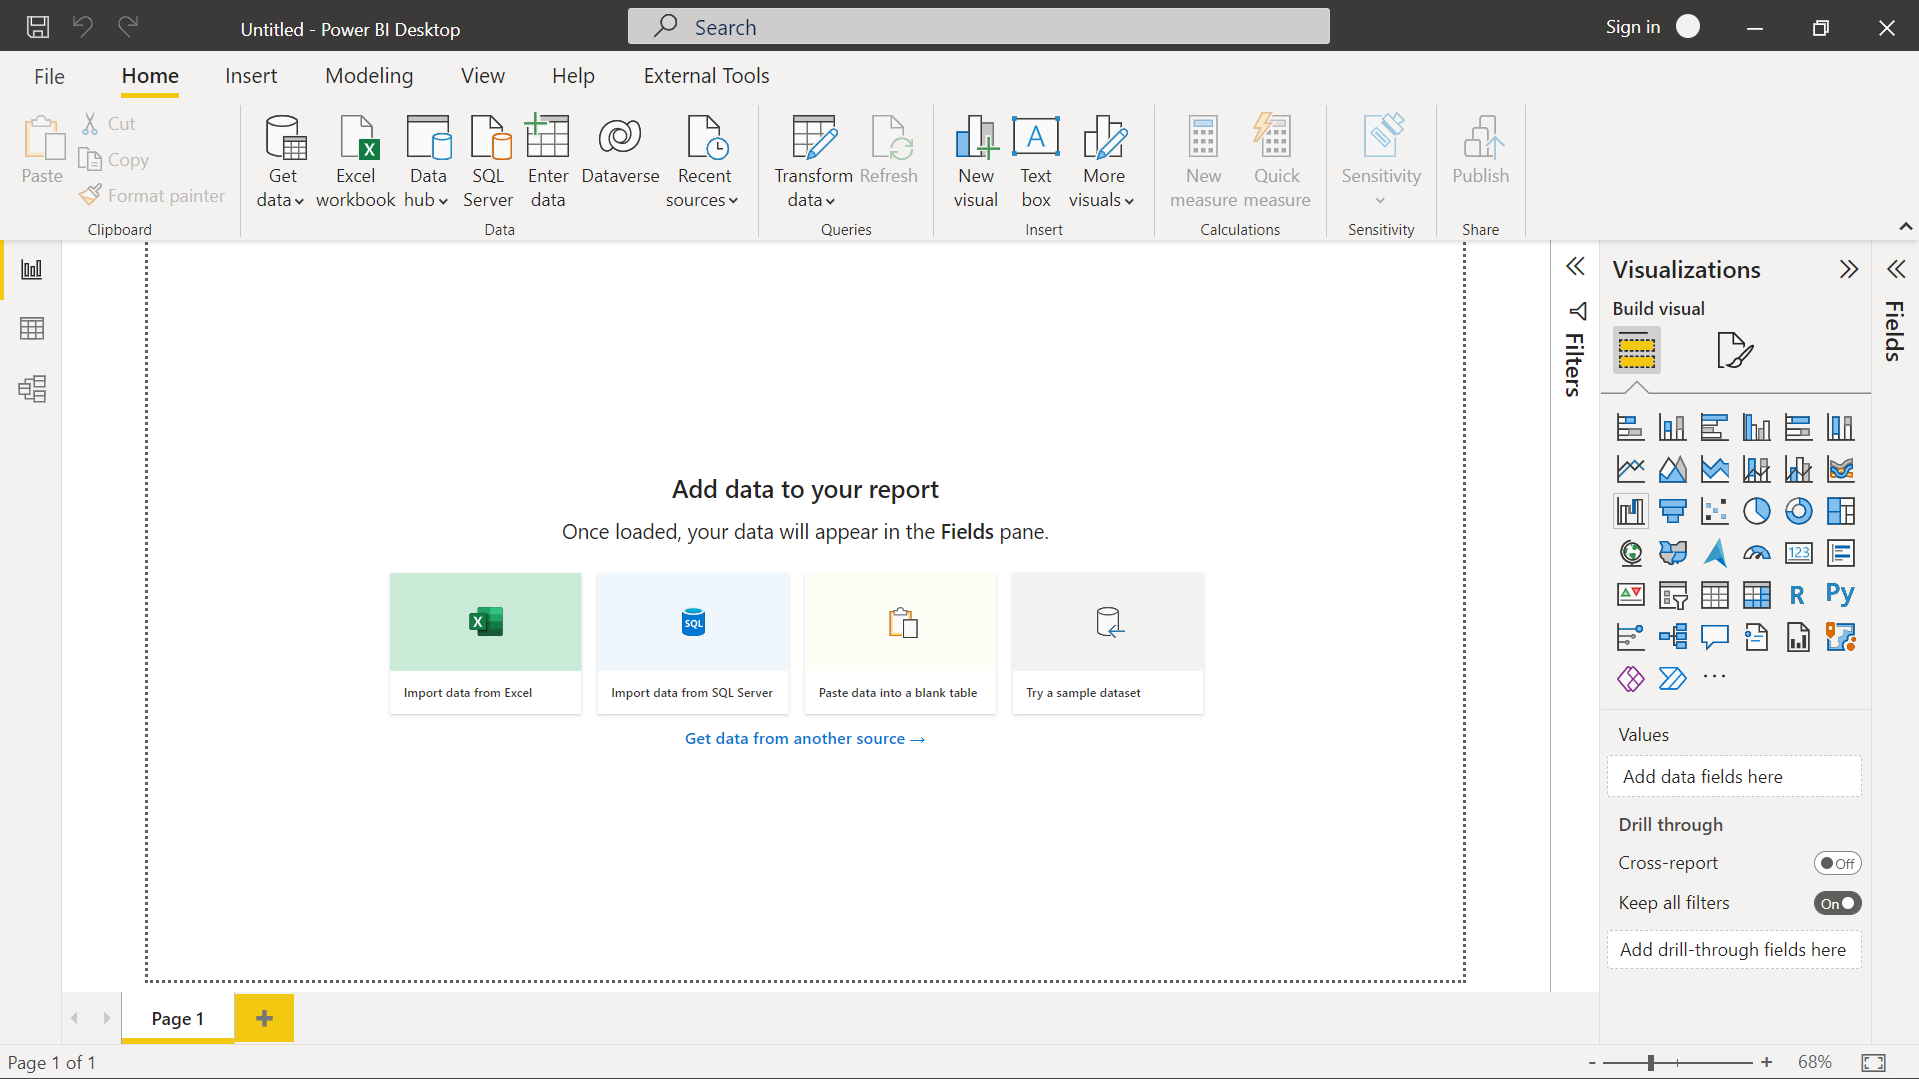
\includegraphics[width=\linewidth,height=4.6cm,keepaspectratio]{ms-learn/lienzo-informe.png}
    \fuente{Usar la vista de informe en Power BI Desktop}{\urlinforme}
    \column{0.37\textwidth}
    \small
    El primer ícono de la izquierda abre la vista \textbf{Informe}. Tiene
    cuatro zonas:
    \begin{itemize}
      \footnotesize
      \item Al centro, el \textbf{lienzo}.
      \item \textbf{Filtros}: lo verás en el paso 11.
      \item \textbf{Visualizaciones}: los íconos de cada tipo de gráfico y,
        debajo, sus casillas (Eje X, Eje Y\ldots).
      \item \textbf{Datos}: tus tablas, con sus columnas y medidas.
    \end{itemize}
    \footnotesize Abajo están las pestañas de las páginas. El signo
    \textbf{+} agrega una página nueva.
  \end{columns}
\end{frame}

\begin{frame}[t]{\npaso{1}\; Prepara el modelo: tiempo y hora}
  \small
  Tres columnas calculadas nuevas (como el paso 17 de la Clase 13): en la
  vista Tabla, clic derecho en la tabla $>$ \menu{Nueva columna}{New
  column}, escribe la fórmula y presiona Enter.
  \vspace{0.05cm}

  \footnotesize
  \renewcommand{\arraystretch}{1.15}
  \begin{tabular}{@{}L{1.9cm}L{7.0cm}L{4.2cm}@{}}
    \toprule
    \textbf{En la tabla} & \textbf{Fórmula} & \textbf{Para qué} \\
    \midrule
    \texttt{Calendario} & \texttt{Inicio de mes = DATE(YEAR(Calendario[Date]), MONTH(Calendario[Date]), 1)} & Un eje de meses que Power BI reconoce como fecha (pasos 8 a 10). \\
    \texttt{Asistencias} & \texttt{hora = HOUR(Asistencias[hora\_entrada])} & La hora de cada entrada, de 0 a 23 (paso 7). \\
    \texttt{Socios} & \texttt{dias\_como\_socio = DATEDIFF(Socios[fecha\_inscripcion], DATE(2026, 9, 30), DAY)} & Días desde la inscripción hasta el corte (paso 12). \\
    \bottomrule
  \end{tabular}

  \vspace{0.15cm}
  \begin{alertblock}{¿Por qué no usar la columna Año-Mes de la Clase 13?}
    \footnotesize \texttt{Año-Mes} es texto, y la línea de tendencia y la
    detección de anomalías solo funcionan con un eje de \textbf{fechas}.
    \texttt{Inicio de mes} es la fecha del día 1 de cada mes.
  \end{alertblock}
\end{frame}

\begin{frame}[t]{\npaso{2}\; Prepara el modelo: la ubicación}
  \small
  El archivo trae la ubicación de dos formas: \textbf{por nombre}
  (\texttt{barrio}, \texttt{municipio}, \texttt{departamento}) y \textbf{por
  coordenadas} (\texttt{latitud}, \texttt{longitud}), en \texttt{Socios} y en
  \texttt{Sedes}.
  \begin{enumerate}
    \footnotesize
    \item En \texttt{Socios}, dos columnas nuevas:
  \end{enumerate}
  \vspace{-0.2cm}
  \codigo{ubicacion = Socios[municipio] \& ", " \& Socios[departamento] \& ", Colombia"\\[2pt]
    banda\_distancia = SWITCH(TRUE(),\\
    \hspace*{1em}Socios[distancia\_sede\_km] < 3, "1. 0 a 3 km",\\
    \hspace*{1em}Socios[distancia\_sede\_km] < 6, "2. 3 a 6 km",\\
    \hspace*{1em}Socios[distancia\_sede\_km] < 10, "3. 6 a 10 km",\\
    \hspace*{1em}"4. 10 km o más")}
  \begin{enumerate}
    \footnotesize
    \setcounter{enumi}{1}
    \item Di a Power BI qué es cada columna: selecciónala y, en
      \menu{Herramientas de columnas}{Column tools} $>$ \menu{Categoría de
      datos}{Data category}, elige \textbf{Latitud} para \texttt{latitud},
      \textbf{Longitud} para \texttt{longitud} (en las dos tablas) y
      \textbf{Lugar} para \texttt{ubicacion}.
  \end{enumerate}
  \guia{Categorización de datos en Power BI Desktop}{\urlcategoria}
  \vspace{-0.1cm}
  \scriptsize \texttt{SWITCH(TRUE(), \ldots)} revisa las condiciones en
  orden y devuelve la primera que se cumple: es la columna condicional
  de la Clase 13, escrita en DAX. El número al inicio ordena las bandas.
\end{frame}

\begin{frame}[t]{\npaso{3}\; Prepara el modelo: medidas y resumen}
  \begin{columns}[T,onlytextwidth]
    \column{0.55\textwidth}
    \small
    Tres medidas nuevas: clic derecho en la tabla $>$ \menu{Nueva
    medida}{New measure}.
    \codigo{Socios = COUNTROWS(Socios)\\[3pt]
      Porcentaje activos = DIVIDE(\\
      \hspace*{1em}CALCULATE(COUNTROWS(Socios),\\
      \hspace*{2em}Socios[activo] = "Sí"),\\
      \hspace*{1em}[Socios])\\[3pt]
      Visitas (con ceros) = COALESCE([Visitas], 0)}
    \footnotesize Crea las dos primeras en \texttt{Socios} y la tercera en
    \texttt{Asistencias}. A \texttt{Porcentaje activos} dale formato de
    porcentaje en la cinta de la medida.
    \column{0.42\textwidth}
    \begin{alertblock}{Que Power BI no sume lo que no se suma}
      \footnotesize Power BI suma solo cualquier columna numérica. Una suma
      de \texttt{id\_socio} o de \texttt{latitud} no tiene sentido. Para
      cada una de esas columnas: \menu{Herramientas de columnas}{Column
      tools} $>$ \menu{Resumen}{Summarization} $>$ \menu{No
      resumir}{Don't summarize}.
    \end{alertblock}
    \footnotesize\textbf{¿Por qué con ceros?} Un día sin entradas no tiene
    filas, y la medida \texttt{Visitas} queda en blanco. \texttt{COALESCE}
    lo cambia por 0, para que una caída se vea en la línea (paso 11).
  \end{columns}
\end{frame}

\begin{frame}[t]{Cómo se crea un objeto visual}
  \begin{columns}[T,onlytextwidth]
    \column{0.47\textwidth}
    \centering
    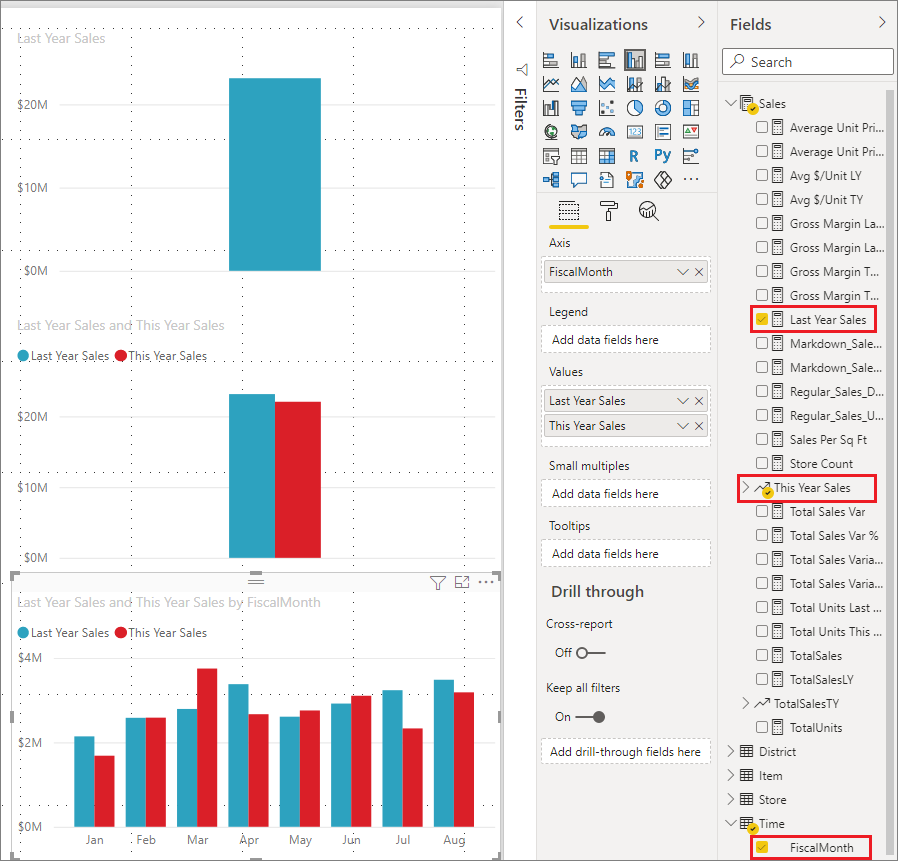
\includegraphics[width=\linewidth,height=4.6cm,keepaspectratio]{ms-learn/agregar-visual.png}
    \fuente{Usar la vista de informe en Power BI Desktop}{\urlinforme}
    \column{0.5\textwidth}
    \small Siempre son los mismos tres movimientos:
    \begin{enumerate}
      \small
      \item Haz clic en un espacio vacío del lienzo y elige el tipo de
        gráfico en el panel \textbf{Visualizaciones}.
      \item Arrastra los campos del panel \textbf{Datos} a las casillas
        (Eje X, Eje Y, Leyenda\ldots).
      \item Cambia el tamaño arrastrando las esquinas del objeto visual.
    \end{enumerate}
    \footnotesize Si eliges un campo antes de elegir el tipo, Power BI
    propone uno. Para cambiarlo, selecciona el objeto visual y haz clic
    en otro ícono de Visualizaciones.\\[3pt]
    Un objeto visual seleccionado se puede borrar con la tecla Supr.
    \guia{Agregar visualizaciones a un informe}{\urlagregar}
  \end{columns}
\end{frame}

\begin{frame}[t]{\npaso{4}\; Tarjetas: los totales primero}
  \begin{columns}[T,onlytextwidth]
    \column{0.5\textwidth}
    \centering
    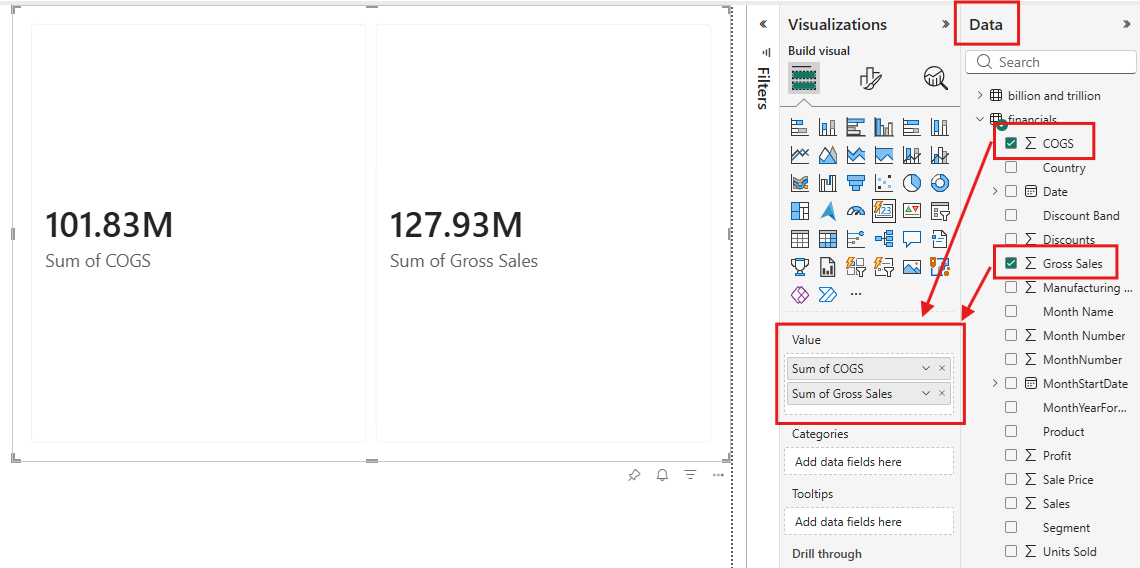
\includegraphics[width=\linewidth,height=3.4cm,keepaspectratio]{ms-learn/tarjeta.png}
    \fuente{Crear un visual de tarjeta en Power BI}{\urltarjeta}
    \vspace{0.05cm}
    \raggedright\footnotesize Empieza siempre por los totales: son la
    referencia contra la que vas a validar todos los demás gráficos.
    \column{0.47\textwidth}
    \small
    \begin{enumerate}
      \small
      \item En Visualizaciones, el ícono \menu{Tarjeta}{Card}.
      \item Arrastra a \menu{Valores}{Values} las medidas
        \texttt{Ingresos}, \texttt{Visitas}, \texttt{Socios} y
        \texttt{Pago promedio}.
    \end{enumerate}
    \footnotesize\textbf{Cifras para comprobar}
    \vspace{0.05cm}

    \scriptsize
    \begin{tabular}{@{}lr@{}}
      \toprule
      Ingresos & 192.424.000 \\
      Visitas & 17.083 \\
      Socios & 300 \\
      Pago promedio & 137.840 \\
      \bottomrule
    \end{tabular}
    \vspace{0.05cm}

    \scriptsize Power BI puede mostrarlas abreviadas (192,42 M) o sin
    puntos de miles: son las mismas cifras.
  \end{columns}
\end{frame}

\begin{frame}[t]{\npaso{5}\; Barras: ingresos por sede}
  \begin{columns}[T,onlytextwidth]
    \column{0.5\textwidth}
    \centering
    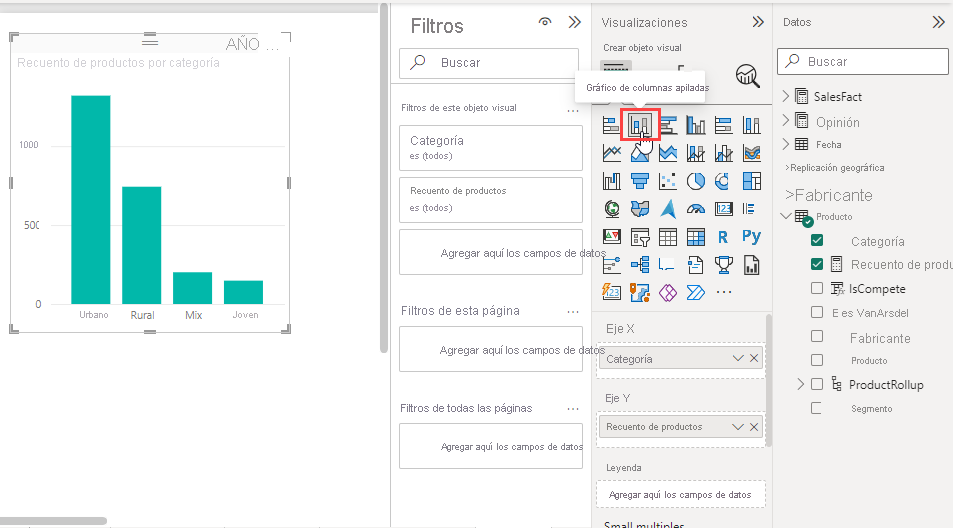
\includegraphics[width=\linewidth,height=2.6cm,keepaspectratio]{ms-learn/cambiar-tipo-visual.png}
    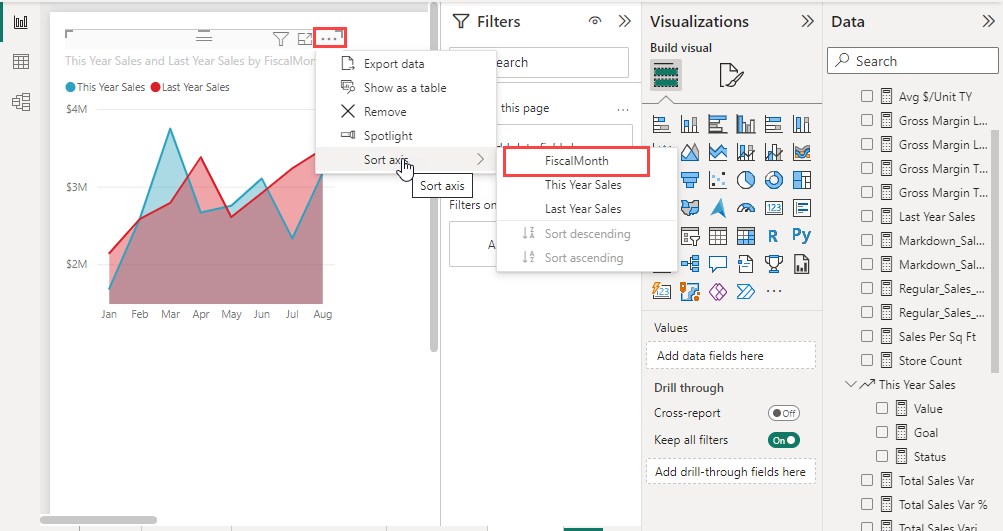
\includegraphics[width=\linewidth,height=2.0cm,keepaspectratio]{ms-learn/ordenar-eje.png}
    \fuente{Agregar visualizaciones a un informe}{\urlagregar}
    \column{0.47\textwidth}
    \small
    \begin{enumerate}
      \footnotesize
      \item Ícono \menu{Gráfico de barras agrupadas}{Clustered bar chart}.
      \item \menu{Eje Y}{Y-axis}: \texttt{Sedes[sede]}. \menu{Eje X}{X-axis}:
        \texttt{Ingresos}.
      \item Ordénalas de mayor a menor: en los tres puntos (\ldots) del
        objeto visual, \menu{Ordenar eje}{Sort axis} $>$
        \texttt{Ingresos} y luego \menu{Orden descendente}{Sort descending}.
    \end{enumerate}
    \footnotesize\textbf{Debes ver}: Poblado 70,8 M; Chapinero 52,5 M;
    Envigado 44,0 M; Itagüí 15,0 M; Cali 10,1 M. La suma es la de la
    tarjeta.
    \begin{alertblock}{¿Barras o columnas?}
      \scriptsize Barras (horizontales) cuando los nombres son largos o
      hay muchas categorías; columnas (verticales) para un eje con orden,
      como las horas.
    \end{alertblock}
  \end{columns}
\end{frame}

\begin{frame}[t]{\npaso{6}\; Formato: los principios de la Clase 11}
  \begin{columns}[T,onlytextwidth]
    \column{0.16\textwidth}
    \centering
    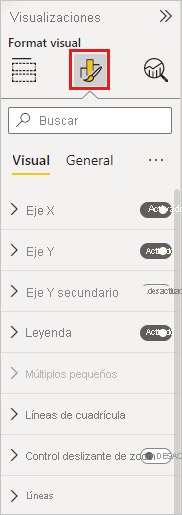
\includegraphics[width=\linewidth,height=4.4cm,keepaspectratio]{ms-learn/panel-formato.png}
    \column{0.36\textwidth}
    \centering
    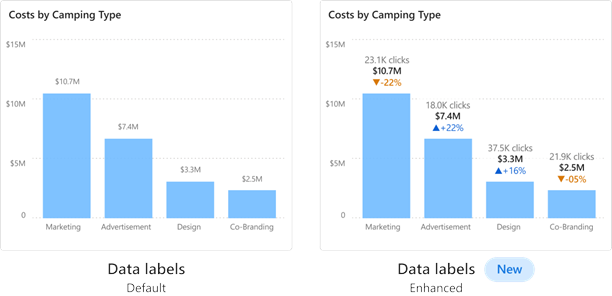
\includegraphics[width=\linewidth,height=2.0cm,keepaspectratio]{ms-learn/etiquetas-datos.png}
    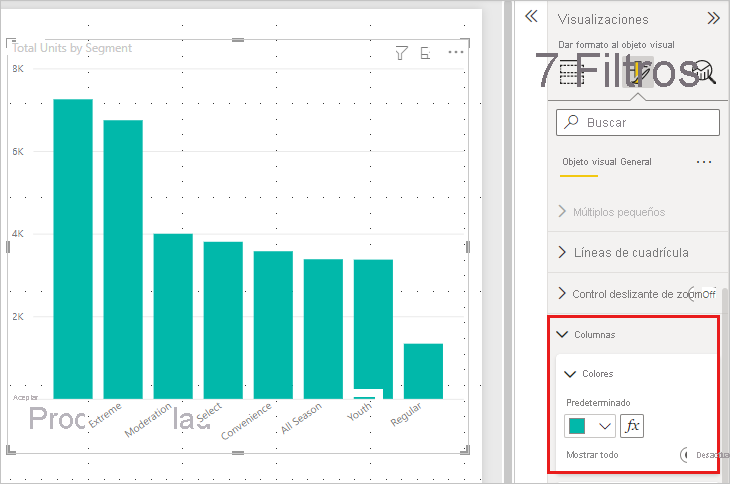
\includegraphics[width=\linewidth,height=2.2cm,keepaspectratio]{ms-learn/colores-datos.png}
    \fuente{Comienza a formatear visualizaciones de informes}{\urlformato}
    \column{0.45\textwidth}
    \small Con el objeto visual seleccionado, el ícono de la brocha abre
    \menu{Formato del objeto visual}{Format visual}:
    \begin{itemize}
      \footnotesize
      \item \textbf{Título}: en \menu{General}{General} $>$
        \menu{Título}{Title}, escribe la conclusión: ``Poblado genera el
        37\% de los ingresos''.
      \item \textbf{Etiquetas de datos}: actívalas, y la escala del eje
        sobra.
      \item \textbf{Color}: un solo color en \menu{Barras}{Bars} $>$
        \menu{Colores}{Colors}. Usa otro solo para destacar lo que importa.
      \item \textbf{Eje en cero}: Power BI lo deja en cero en las barras;
        no lo cambies.
    \end{itemize}
  \end{columns}
\end{frame}

\begin{frame}[t]{\npaso{7}\; Columnas: ¿a qué hora se llena el gimnasio?}
  \begin{columns}[T,onlytextwidth]
    \column{0.47\textwidth}
    \centering
    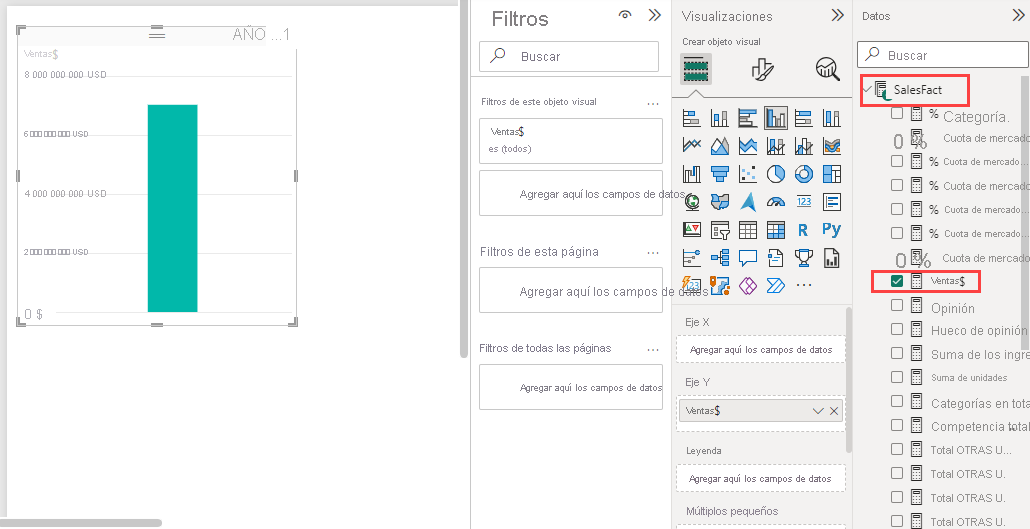
\includegraphics[width=\linewidth,height=3.3cm,keepaspectratio]{ms-learn/visual-primer-campo.png}
    \fuente{Agregar visualizaciones a un informe}{\urlagregar}
    \vspace{0.05cm}
    \footnotesize\raggedright Si en el eje aparecen los números de hora
    desordenados, en los tres puntos elige \menu{Ordenar eje}{Sort axis}
    $>$ \texttt{hora} y orden ascendente.
    \column{0.5\textwidth}
    \small
    \begin{enumerate}
      \footnotesize
      \item Ícono \menu{Gráfico de columnas agrupadas}{Clustered column
        chart}.
      \item \menu{Eje X}{X-axis}: \texttt{Asistencias[hora]}.
        \menu{Eje Y}{Y-axis}: \texttt{Visitas}.
    \end{enumerate}
    \footnotesize\textbf{Qué debes ver}: dos picos, de 6 a 8 a.\,m. (unas
    2000 visitas por hora) y de 5 a 8 p.\,m. (unas 1900), y un mediodía con
    la mitad.

    \vspace{0.1cm}
    \scriptsize
    \begin{tabular}{@{}lrr@{}}
      \toprule
      \textbf{Franja} & \textbf{Visitas} & \textbf{Del total} \\
      \midrule
      Mañana (5 a 9 a.\,m.) & 6742 & 39,5\% \\
      Mediodía (11 a.\,m. a 3 p.\,m.) & 2578 & 15,1\% \\
      Tarde (5 a 10 p.\,m.) & 7763 & 45,4\% \\
      \bottomrule
    \end{tabular}
  \end{columns}
\end{frame}

% ============================================================
\section{Hora 2: Tiempo, anomalías, relación y lugar}
% ============================================================
\begin{frame}[t]{\npaso{8}\; Línea: los ingresos mes a mes}
  \begin{columns}[T,onlytextwidth]
    \column{0.52\textwidth}
    \centering
    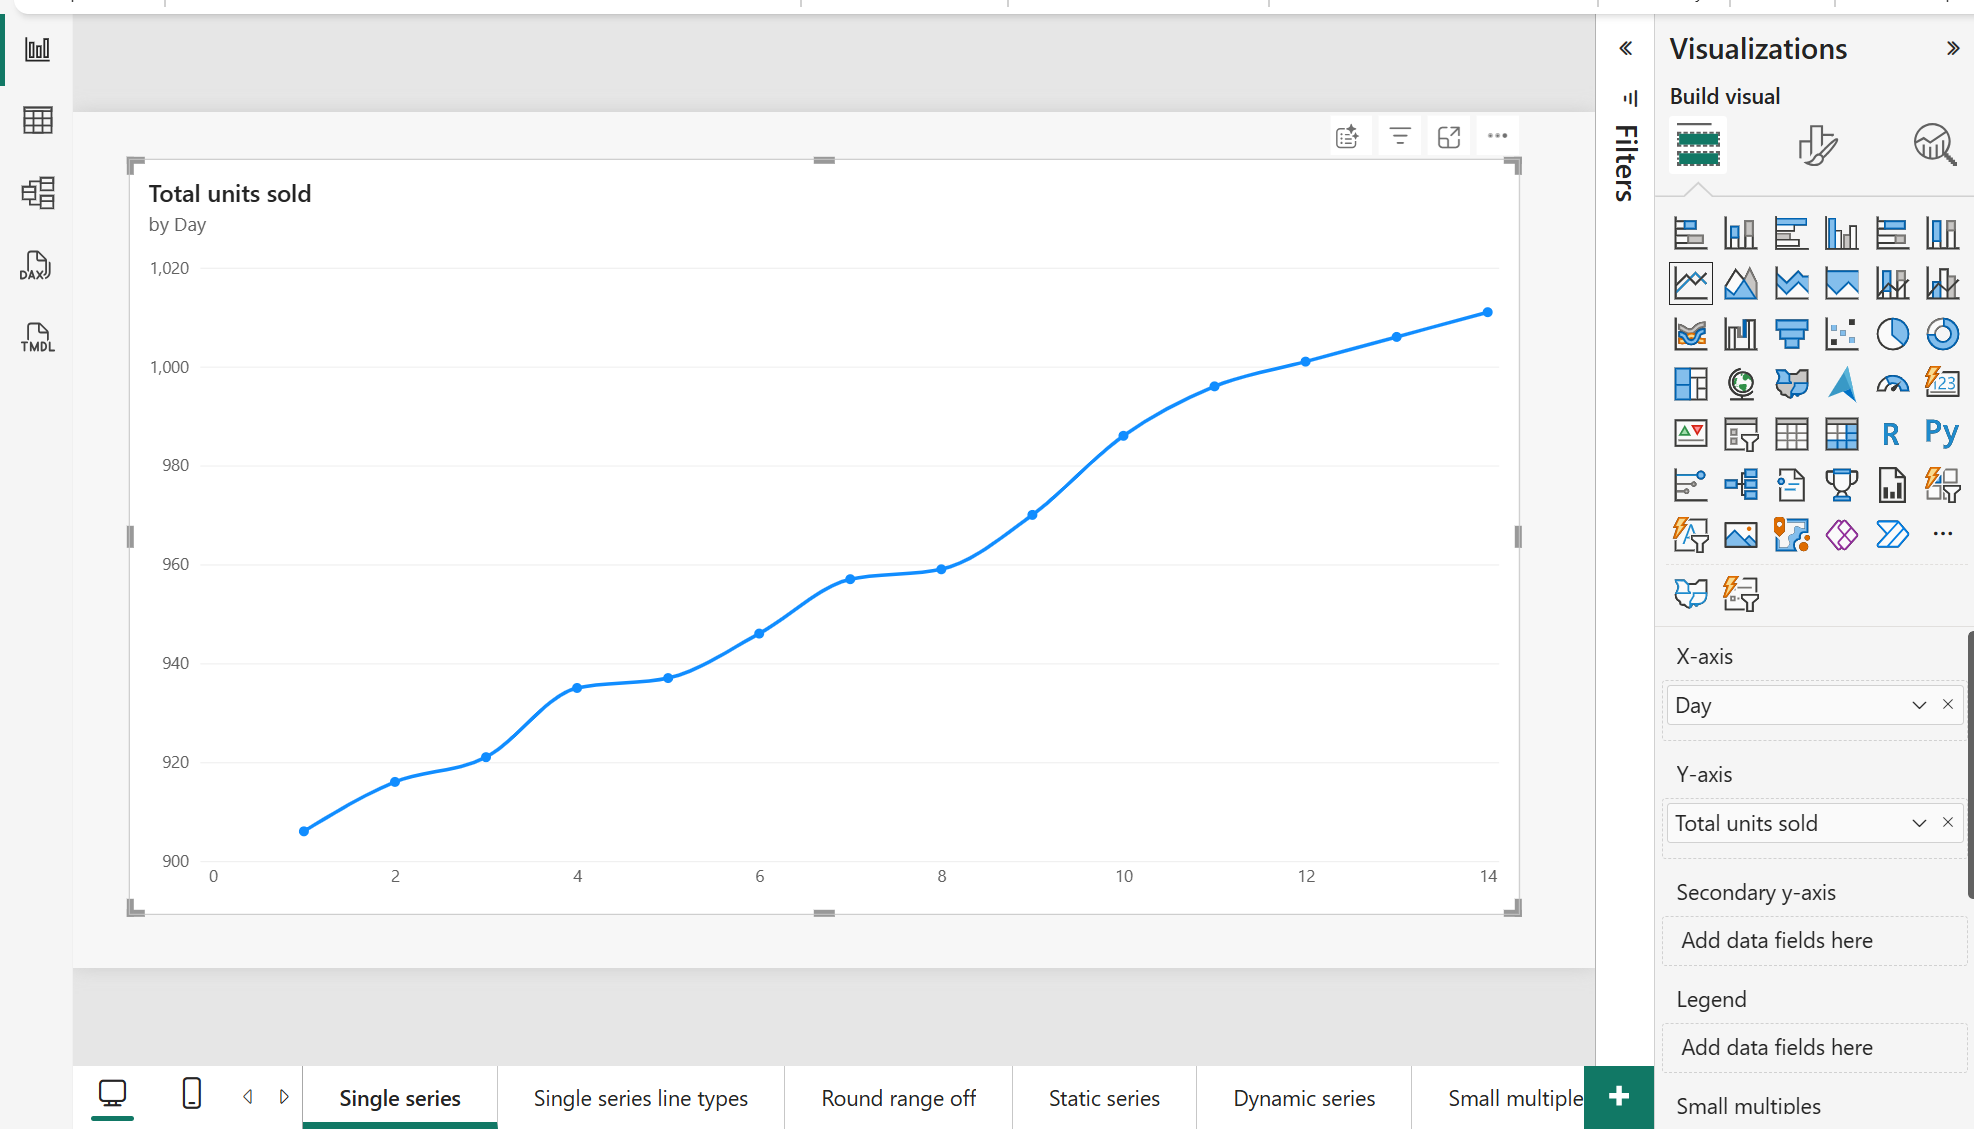
\includegraphics[width=\linewidth,height=3.5cm,keepaspectratio]{ms-learn/linea-una-serie.png}
    \fuente{Gráficos de líneas en Power BI}{\urllineas}
    \column{0.45\textwidth}
    \small
    \begin{enumerate}
      \footnotesize
      \item Ícono \menu{Gráfico de líneas}{Line chart}.
      \item \menu{Eje X}{X-axis}: \texttt{Calendario[Inicio de mes]}.
        \menu{Eje Y}{Y-axis}: \texttt{Ingresos}.
      \item En Formato $>$ \menu{Eje X}{X-axis}, revisa que el tipo sea
        \menu{Continuo}{Continuous}.
    \end{enumerate}
    \footnotesize\textbf{Debes ver} una línea que sube de 4,65 M (sep
    2025) a 23,15 M (sep 2026).
    \begin{alertblock}{Una línea es para el tiempo}
      \scriptsize Úsala cuando el eje tiene orden: meses, días, horas. Para
      comparar sedes o planes, usa barras (Clase 11).
    \end{alertblock}
  \end{columns}
\end{frame}

\begin{frame}[t]{\npaso{9}\; La línea de tendencia}
  \begin{columns}[T,onlytextwidth]
    \column{0.42\textwidth}
    \centering
    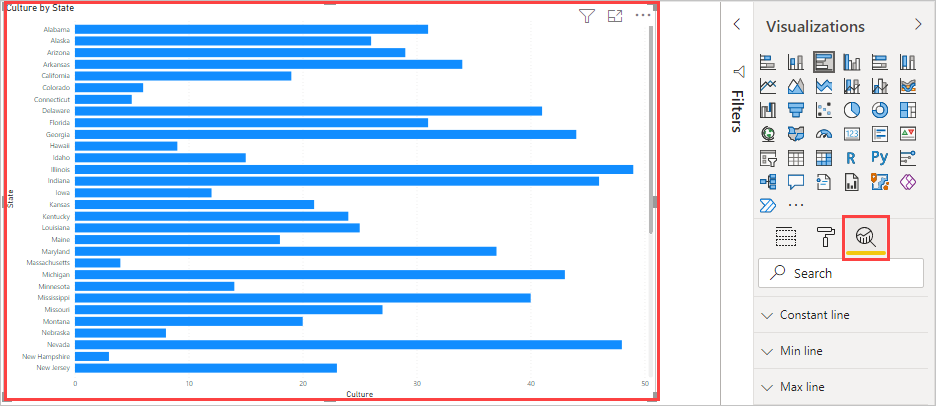
\includegraphics[width=\linewidth,height=2.6cm,keepaspectratio]{ms-learn/icono-analisis.png}
    \fuente{Uso del panel Análisis en Power BI}{\urlanalisis}
    \column{0.14\textwidth}
    \centering
    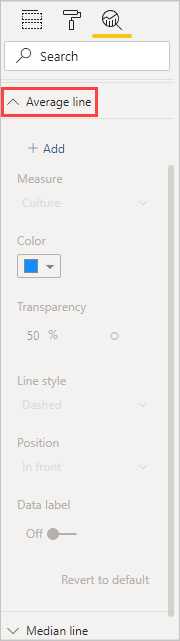
\includegraphics[width=\linewidth,height=4.2cm,keepaspectratio]{ms-learn/opciones-analisis.png}
    \column{0.41\textwidth}
    \small
    \begin{enumerate}
      \footnotesize
      \item Selecciona la línea del paso 8.
      \item En Visualizaciones, el tercer ícono (una lupa sobre un
        gráfico): panel \menu{Análisis}{Analytics}.
      \item Abre \menu{Línea de tendencia}{Trend line} $>$
        \menu{Agregar}{Add}.
    \end{enumerate}
    \footnotesize\textbf{Cómo se lee}: la tendencia es la recta que mejor
    resume la serie. Aquí sube, pero mira los últimos meses: mayo 22,2 M,
    junio 18,9 M, julio 20,6 M, agosto 22,9 M y septiembre 23,2 M. El
    crecimiento parece frenarse desde mayo.

    \vspace{0.05cm}
    \scriptsize En el mismo panel están las líneas de promedio, mínimo y
    máximo.
  \end{columns}
\end{frame}

\begin{frame}[t]{\npaso{10}\; Comparar en el tiempo: una línea por sede}
  \begin{columns}[T,onlytextwidth]
    \column{0.52\textwidth}
    \centering
    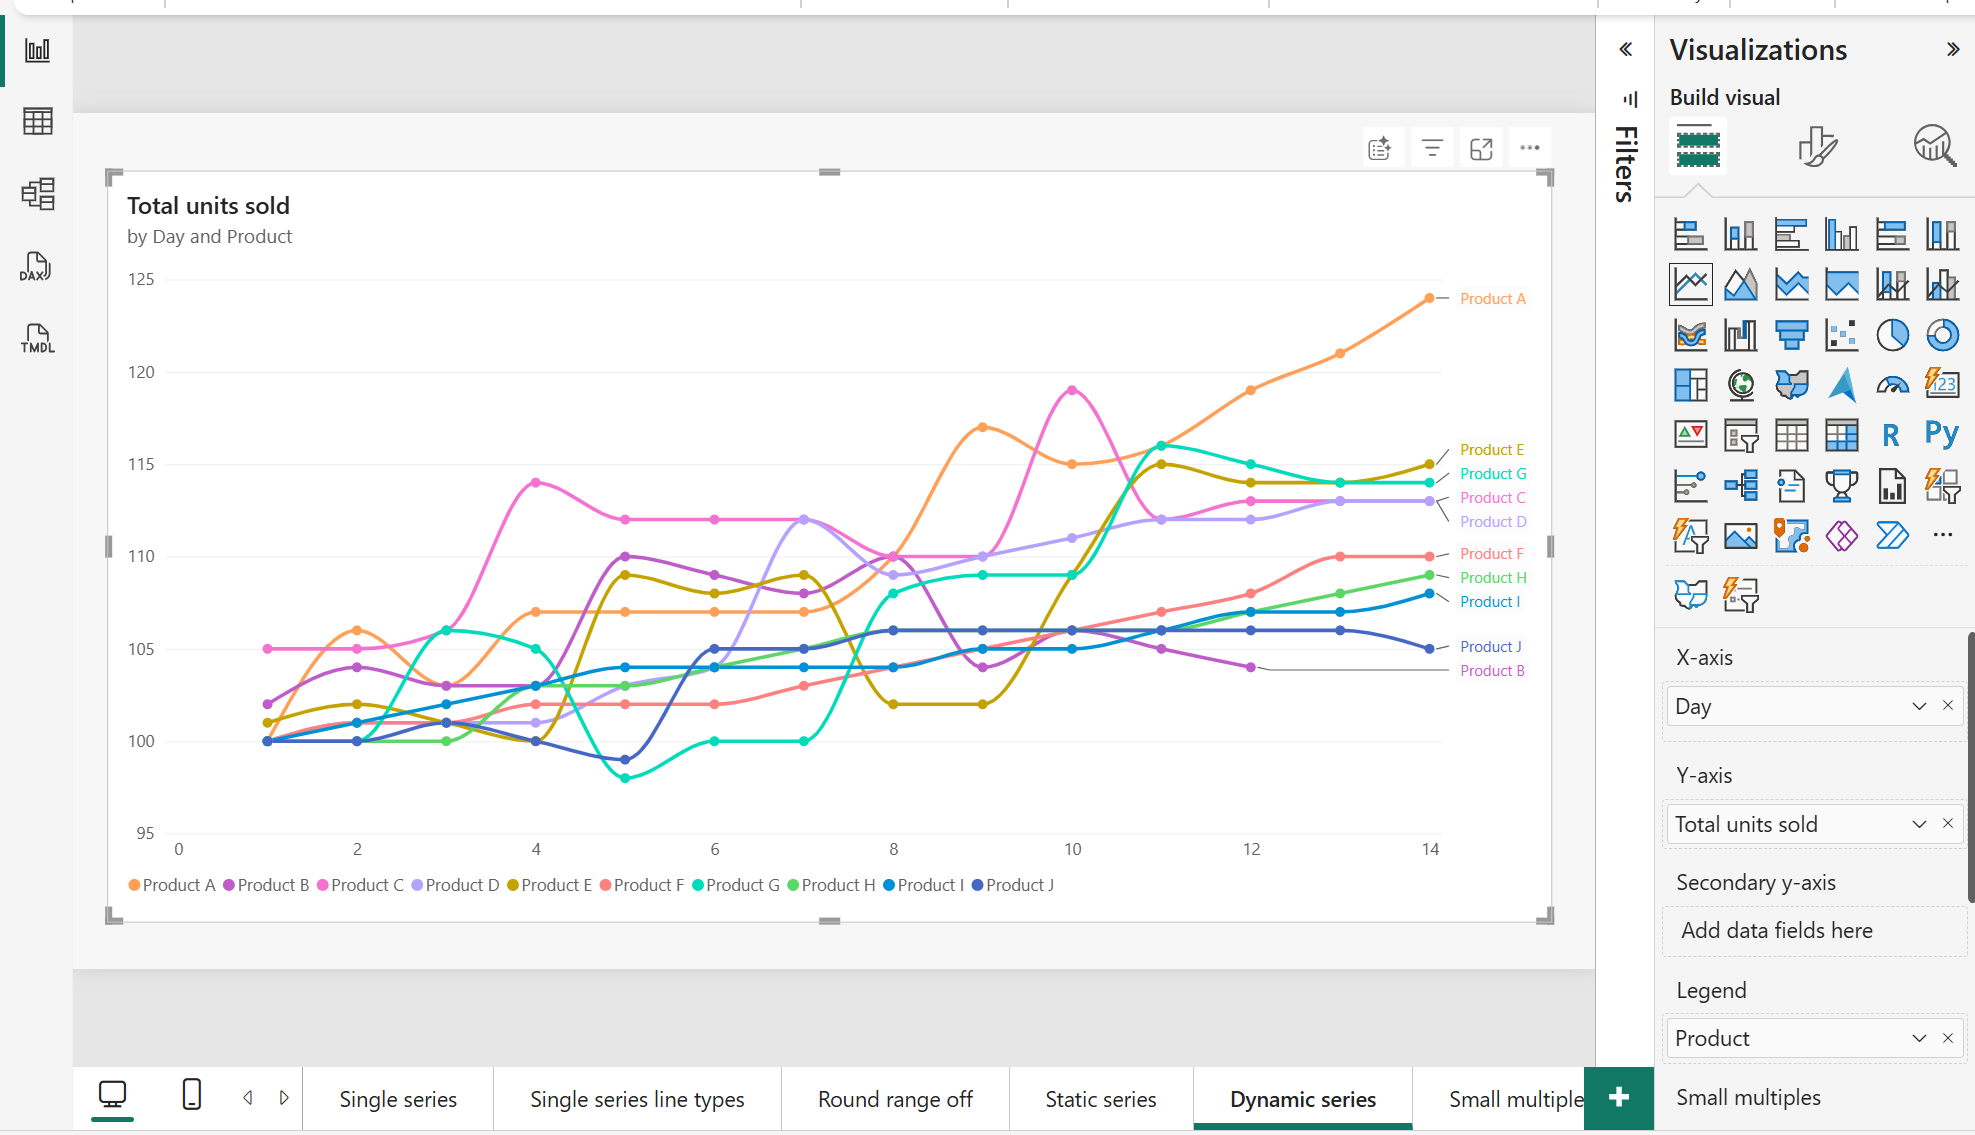
\includegraphics[width=\linewidth,height=3.5cm,keepaspectratio]{ms-learn/linea-varias-series.png}
    \fuente{Gráficos de líneas en Power BI}{\urllineas}
    \column{0.45\textwidth}
    \small
    \begin{enumerate}
      \footnotesize
      \item Otro \menu{Gráfico de líneas}{Line chart}, con
        \texttt{Calendario[Inicio de mes]} en el Eje X y \texttt{Visitas}
        en el Eje Y.
      \item Arrastra \texttt{Sedes[sede]} a \menu{Leyenda}{Legend}: una
        línea por sede.
    \end{enumerate}
    \footnotesize\textbf{Qué buscar}:
    \begin{itemize}
      \scriptsize
      \item Cali empieza en marzo de 2026, cuando abrió.
      \item Envigado cae en junio (330 visitas, frente a 408 en mayo y 435
        en julio) y luego se recupera. Las demás sedes no caen ese mes.
    \end{itemize}
    \scriptsize Comparar una serie contra las otras te dice si un cambio
    es de todo el negocio o de una sola parte.
  \end{columns}
\end{frame}

\begin{frame}[t]{¿Qué es una anomalía?}
  \small
  Un valor que se sale de lo que esperabas según el resto de la serie: un
  pico o una caída repentina. Ante una anomalía hay siempre dos
  preguntas:
  \vspace{0.15cm}
  \begin{columns}[T,onlytextwidth]
    \column{0.48\textwidth}
    \begin{alertblock}{¿Es un error en los datos?}
      \small Un archivo que no se cargó, un sistema que dejó de registrar
      o un duplicado. Se corrige en la fuente o en Power Query.
    \end{alertblock}
    \column{0.48\textwidth}
    \begin{exampleblock}{¿Es algo que pasó de verdad?}
      \small Un cierre, una promoción o un día festivo. No se corrige: se
      explica, y puede ser un insight.
    \end{exampleblock}
  \end{columns}
  \vspace{0.2cm}
  \small Los datos solos no te dicen cuál de las dos es: hay que preguntar
  a quien conoce la operación. Nunca borres una anomalía para que el
  gráfico se vea mejor.
\end{frame}

\begin{frame}[t]{\npaso{11}\; Buscar la anomalía de Envigado, día a día}
  \begin{columns}[T,onlytextwidth]
    \column{0.44\textwidth}
    \centering
    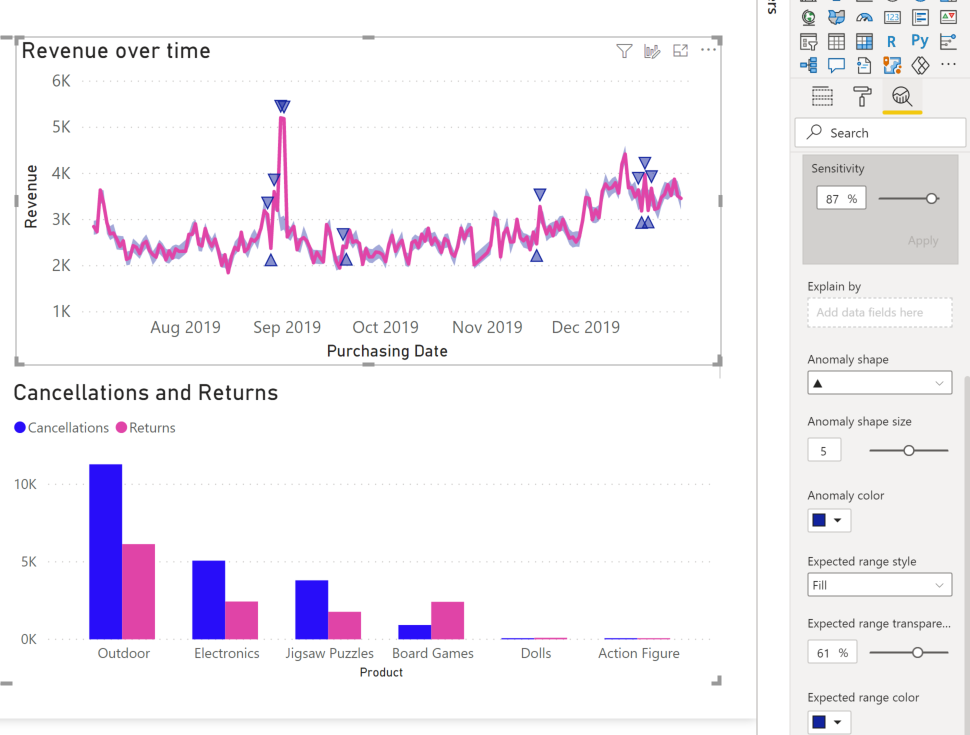
\includegraphics[width=\linewidth,height=3.5cm,keepaspectratio]{ms-learn/anomalias-formato.png}
    \fuente{Tutorial de detección de anomalías para Power BI}{\urlanomalias}
    \column{0.53\textwidth}
    \footnotesize
    \begin{enumerate}
      \footnotesize
      \item Un \menu{Gráfico de líneas}{Line chart} con
        \texttt{Calendario[Date]} en el Eje X y \texttt{Visitas (con ceros)}
        en el Eje Y.
      \item Solo para Envigado: en el panel \menu{Filtros}{Filters},
        arrastra \texttt{Sedes[sede]} a \menu{Filtros en este objeto
        visual}{Filters on this visual} y marca \textit{Sede Envigado}.
      \item Panel \menu{Análisis}{Analytics} $>$ \menu{Buscar
        anomalías}{Find anomalies} $>$ \menu{Agregar}{Add}.
    \end{enumerate}
    \textbf{Debes ver} unas 15 visitas diarias en junio y una caída a
    \textbf{0 del 8 al 14 de junio de 2026}. La detección automática marca
    los puntos fuera del rango esperado; si no marca esos días, sube la
    \menu{Sensibilidad}{Sensitivity}.
    \vspace{0.05cm}

    \scriptsize El filtro solo afecta a este objeto visual. Los filtros se
    ven a fondo en la Clase 15
    (\href{\urlfiltros}{\color{esumerOrange}guía oficial de filtros}).
  \end{columns}
\end{frame}

\begin{frame}[t]{La anomalía de Envigado: ¿error o realidad?}
  \small
  Siete días seguidos con cero entradas en una sede que recibe unas 15
  diarias no es azar. Antes de concluir, valida:
  \vspace{0.1cm}
  \begin{enumerate}
    \small
    \item \textbf{¿Pasa en todas las sedes?} No: solo Envigado (paso 10).
      Entonces no es un problema de todo el sistema.
    \item \textbf{¿Hay pagos esos días?} Sí: Envigado tuvo 34 pagos en
      junio (36 en mayo, 33 en julio) y 7 en esa misma semana. Los socios no
      se fueron.
    \item \textbf{¿Qué dice la operación?} Al preguntar, la sede confirma
      que \textbf{cerró por mantenimiento} esa semana.
  \end{enumerate}
  \vspace{0.1cm}
  \begin{exampleblock}{El insight}
    \small La caída de junio en Envigado es un cierre, no una pérdida de
    demanda. Recomendación: avisar los cierres con anticipación, ofrecer
    la Sede Poblado (a unos 5 km) mientras dure, y registrar los cierres
    en los datos para que nadie los confunda con una caída de socios.
  \end{exampleblock}
\end{frame}

\begin{frame}[t]{\npaso{12}\; Dispersión: antigüedad y visitas}
  \begin{columns}[T,onlytextwidth]
    \column{0.3\textwidth}
    \centering
    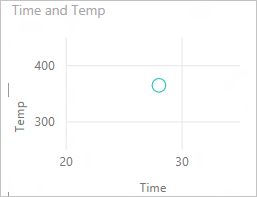
\includegraphics[width=\linewidth,height=2.6cm,keepaspectratio]{ms-learn/dispersion-un-punto.png}
    \fuente{Gráficos de dispersión, burbujas y trazados de puntos}{\urldispersion}
    \vspace{0.05cm}
    \raggedright\scriptsize\textbf{¿Ves un solo punto, como aquí?} Falta
    \texttt{id\_socio} en Valores: sin él, Power BI junta todo en un punto.
    \column{0.67\textwidth}
    \small
    \begin{enumerate}
      \footnotesize
      \item Ícono \menu{Gráfico de dispersión}{Scatter chart}.
      \item \menu{Valores}{Values}: \texttt{Socios[id\_socio]}, para que
        cada punto sea un socio.
      \item \menu{Eje X}{X-axis}: \texttt{Socios[dias\_como\_socio]}.
        \menu{Eje Y}{Y-axis}: \texttt{Visitas}.
      \item \menu{Leyenda}{Legend}: \texttt{Socios[activo]}.
    \end{enumerate}
    \footnotesize\textbf{Cómo se lee}: 300 puntos, uno por socio. Los que
    llevan más tiempo tienen más visitas (correlación de 0,63): es lo
    esperable. Lo interesante son los puntos \textbf{por debajo} de la
    nube: socios que vienen menos de lo que su antigüedad haría esperar.
    La mayoría son inactivos.
    \vspace{0.05cm}

    \footnotesize Los socios activos venían en promedio \textbf{2,16 veces
    por semana}; los inactivos, \textbf{1,63}.
  \end{columns}
\end{frame}

\begin{frame}[t]{Cuatro usos de los mapas}
  \small
  Un mapa responde a una sola pregunta: \textbf{¿dónde?} Hoy lo usamos de
  cuatro formas:
  \vspace{0.1cm}

  \footnotesize
  \renewcommand{\arraystretch}{1.2}
  \begin{tabular}{@{}L{0.6cm}L{3.8cm}L{4.1cm}L{4.0cm}@{}}
    \toprule
    & \textbf{Pregunta} & \textbf{Cómo se ubica el dato} & \textbf{Campos} \\
    \midrule
    \npaso{13} & ¿Dónde están las sedes y cuánto genera cada una? & coordenadas de la sede & \texttt{Sedes[latitud]}, \texttt{Sedes[longitud]} \\
    \npaso{14} & ¿Dónde viven los socios activos e inactivos? & coordenadas del socio & \texttt{Socios[latitud]}, \texttt{Socios[longitud]} \\
    \npaso{15} & ¿Cuántos socios hay por municipio? & \textbf{por nombre}: Power BI geocodifica & \texttt{Socios[ubicacion]} \\
    \npaso{16} & ¿Los que viven lejos se retiran más? & sin mapa: barras por distancia & \texttt{Socios[banda\_distancia]} \\
    \bottomrule
  \end{tabular}

  \vspace{0.15cm}
  \begin{alertblock}{Usa el objeto visual Azure Maps}
    \footnotesize Microsoft anunció que los mapas antiguos de Bing
    (\textit{Mapa} y \textit{Mapa coroplético}) dejarán de estar
    disponibles, y recomienda Azure Maps. Los mapas necesitan internet: los
    datos de ubicación se envían al servicio de mapas de Microsoft.
  \end{alertblock}
\end{frame}

\begin{frame}[t]{\npaso{13}\; Mapa de sedes, por coordenadas}
  \small
  \begin{enumerate}
    \small
    \item En Visualizaciones, el ícono \menu{Azure Maps}{Azure Maps}.
    \item \menu{Latitud}{Latitude}: \texttt{Sedes[latitud]}.
      \menu{Longitud}{Longitude}: \texttt{Sedes[longitud]}.
    \item \menu{Tamaño}{Size}: \texttt{Ingresos}. \menu{Leyenda}{Legend}:
      \texttt{Sedes[sede]}.
  \end{enumerate}
  \vspace{0.05cm}
  \begin{columns}[T,onlytextwidth]
    \column{0.5\textwidth}
    \footnotesize\textbf{Qué debes ver}: cinco burbujas. Tres casi juntas
    en el Valle de Aburrá (Poblado, Envigado e Itagüí, a menos de 5 km
    entre sí), una en Bogotá y una en Cali. Acércate con la rueda del
    ratón para separarlas.
    \column{0.47\textwidth}
    \begin{alertblock}{Si el mapa no se dibuja}
      \scriptsize Revisa la conexión a internet. Si no aparece el ícono de
      Azure Maps o pide habilitarlo, en algunos equipos institucionales
      tiene que activarlo el administrador; mientras tanto, usa el objeto
      visual \menu{Mapa}{Map}.
    \end{alertblock}
  \end{columns}
  \vspace{0.05cm}
  \footnotesize\textbf{El dato}: las tres sedes del Valle de Aburrá
  generan 129,9 M de los 192,4 M (\textbf{67,5\%}); Bogotá, el 27,3\%;
  Cali, el 5,3\%, pero abrió en marzo.
  \guia{Comienza con la visualización de Azure Maps en Power BI}{\urlazuremaps}
\end{frame}

\begin{frame}[t]{\npaso{14}\; Mapa de socios: dónde viven}
  \small
  \begin{enumerate}
    \small
    \item Otro objeto visual \menu{Azure Maps}{Azure Maps}.
    \item \menu{Latitud}{Latitude}: \texttt{Socios[latitud]}.
      \menu{Longitud}{Longitude}: \texttt{Socios[longitud]}.
    \item \menu{Leyenda}{Legend}: \texttt{Socios[activo]}. Así cada punto
      es un socio, coloreado según si sigue activo.
  \end{enumerate}
  \vspace{0.05cm}
  \begin{columns}[T,onlytextwidth]
    \column{0.5\textwidth}
    \footnotesize\textbf{Qué buscar}: acércate a cada ciudad. Los puntos
    de socios activos se agrupan cerca de las sedes; los de inactivos
    aparecen más hacia afuera: Bello, Caldas o Robledo en Antioquia, Suba
    y Kennedy en Bogotá, Jamundí en el sur de Cali.
    \column{0.47\textwidth}
    \begin{alertblock}{Un mapa sugiere, no demuestra}
      \scriptsize Con puntos encimados es fácil ver lo que uno espera ver.
      Lo que el mapa sugiere se confirma con cifras: eso es el paso 16.
    \end{alertblock}
  \end{columns}
  \vspace{0.1cm}
  \footnotesize Las coordenadas son aproximadas (el centro de cada barrio,
  con un pequeño desplazamiento por socio): sirven para ver patrones, no
  para ubicar a una persona.
\end{frame}

\begin{frame}[t]{\npaso{15}\; Mapa por nombre: Power BI adivina}
  \small
  Sin coordenadas, el mapa convierte el \textbf{nombre} del lugar en un
  punto (geocodificar). Pruébalo:
  \begin{enumerate}
    \footnotesize
    \item Un \menu{Azure Maps}{Azure Maps} con \menu{Ubicación}{Location}:
      \texttt{Socios[municipio]} y \menu{Tamaño}{Size}: \texttt{Socios}.
    \item Mira dónde quedó cada burbuja. Un nombre solo puede ser
      ambiguo: \textbf{Caldas} es un municipio de Antioquia, pero también
      un departamento del Eje Cafetero. Si ves una burbuja cerca de
      Manizales, Power BI eligió el equivocado.
    \item Cambia la ubicación por \texttt{Socios[ubicacion]}
      (\texttt{"Caldas, Antioquia, Colombia"}), que creaste en el paso 2.
  \end{enumerate}
  \begin{columns}[T,onlytextwidth]
    \column{0.48\textwidth}
    \begin{exampleblock}{Por nombre}
      \scriptsize Fácil cuando solo tienes ciudades o países. Escribe
      siempre el nombre completo (municipio, departamento, país) y marca la
      categoría de datos (paso 2).
    \end{exampleblock}
    \column{0.48\textwidth}
    \begin{exampleblock}{Por coordenadas}
      \scriptsize Exacto y sin ambigüedad, pero alguien tiene que haber
      guardado la latitud y la longitud de cada registro.
    \end{exampleblock}
  \end{columns}
\end{frame}

\begin{frame}[t]{\npaso{16}\; Confirmar con cifras: activos según la distancia}
  \begin{columns}[T,onlytextwidth]
    \column{0.5\textwidth}
    \small
    \begin{enumerate}
      \footnotesize
      \item \menu{Gráfico de columnas agrupadas}{Clustered column chart}.
      \item \menu{Eje X}{X-axis}: \texttt{Socios[banda\_distancia]}.
        \menu{Eje Y}{Y-axis}: \texttt{Porcentaje activos}.
      \item Agrega \texttt{Socios} en \menu{Información sobre
        herramientas}{Tooltips}: al pasar el ratón verás cuántos socios
        hay en cada banda.
    \end{enumerate}
    \footnotesize Así confirmas con números lo que el mapa del paso 14
    sugería.
    \column{0.47\textwidth}
    \footnotesize\textbf{Debes ver}
    \vspace{0.05cm}

    \scriptsize
    \begin{tabular}{@{}lrr@{}}
      \toprule
      \textbf{Distancia a la sede} & \textbf{Socios} & \textbf{Activos} \\
      \midrule
      0 a 3 km & 122 & 89,3\% \\
      3 a 6 km & 87 & 86,2\% \\
      6 a 10 km & 45 & 60,0\% \\
      10 km o más & 46 & 63,0\% \\
      \midrule
      \textbf{Total} & \textbf{300} & \textbf{80,0\%} \\
      \bottomrule
    \end{tabular}
    \vspace{0.1cm}

    \footnotesize A menos de 6 km sigue activo el \textbf{88,0\%}; a 6 km o
    más, solo el \textbf{61,5\%}. Y 35 de los 60 inactivos viven a 6 km o
    más, aunque ahí vive menos de un tercio de los socios.
  \end{columns}
\end{frame}

% ============================================================
\section{Hora 3: Del gráfico al insight}
% ============================================================
\begin{frame}[t]{¿Qué es un insight?}
  \small
  Un insight no es un gráfico ni un número: es una frase que alguien que
  decide puede usar. Tiene cuatro partes (las mismas de la ficha de la
  Clase 12):
  \vspace{0.2cm}
  \begin{center}
  \begin{tikzpicture}[
    pieza/.style={draw=esumerNavy,line width=0.7pt,rounded corners=3pt,fill=white,
                  minimum width=3.1cm,text width=2.9cm,minimum height=1.6cm,align=center,inner sep=3pt},
    tit/.style={font=\bfseries\scriptsize,text=white,fill=esumerTeal,rounded corners=2pt,
                minimum width=3.1cm,inner sep=2pt},
    flecha/.style={-{Stealth[length=2.4mm]},line width=1pt,color=esumerNavy},
  ]
    \foreach \x/\tit in {0/Evidencia, 3.55/Hallazgo, 7.1/Por qué importa, 10.65/Recomendación}
      {\node[tit] at (\x,1.15) {\tit};}
    \node[pieza] (a) at (0,0) {\scriptsize Columnas por hora: 15\% de las visitas al mediodía};
    \node[pieza] (b) at (3.55,0) {\scriptsize El gimnasio está casi vacío de 11 a.\,m. a 3 p.\,m.};
    \node[pieza] (c) at (7.1,0) {\scriptsize Se paga personal y espacio que casi nadie usa};
    \node[pieza] (d) at (10.65,0) {\scriptsize Clases grupales y un plan con descuento al mediodía};
    \foreach \u/\v in {a/b, b/c, c/d} {\draw[flecha] (\u) -- (\v);}
  \end{tikzpicture}
  \end{center}
  \vspace{0.2cm}
  \small Si a tu hallazgo le falta la recomendación, todavía es una
  \textbf{observación}. Si le falta la evidencia, es una \textbf{opinión}.
\end{frame}

\begin{frame}[t]{¿Accionable o curiosidad?}
  \small
  Antes de poner un hallazgo en la ficha, hazle estas tres preguntas:
  \vspace{0.1cm}
  \begin{enumerate}
    \small
    \item \textbf{¿Cambia una decisión?} Si nadie haría nada distinto al
      saberlo, es una curiosidad.
    \item \textbf{¿Alguien puede actuar?} Una recomendación debe tener un
      responsable posible: la sede, mercadeo, el área de retención.
    \item \textbf{¿Es sólido?} ¿Pasó la validación de la diapositiva
      siguiente?
  \end{enumerate}
  \vspace{0.1cm}
  \begin{columns}[T,onlytextwidth]
    \column{0.48\textwidth}
    \begin{alertblock}{Curiosidad}
      \footnotesize ``Las visitas son casi iguales todos los días de la
      semana.'' Es cierto, pero no sugiere ninguna acción.
    \end{alertblock}
    \column{0.48\textwidth}
    \begin{exampleblock}{Accionable}
      \footnotesize ``Los socios que viven a 6 km o más se retiran más del
      triple (38,5\% frente a 12,0\%).'' Sugiere dónde captar socios y a
      quién acompañar.
    \end{exampleblock}
  \end{columns}
\end{frame}

\begin{frame}[t]{Validar las cifras: cinco preguntas}
  \footnotesize
  \renewcommand{\arraystretch}{1.2}
  \begin{tabular}{@{}L{3.6cm}L{9.6cm}@{}}
    \toprule
    \textbf{Pregunta} & \textbf{Ejemplo con nuestros datos} \\
    \midrule
    1. ¿Los totales cuadran? & La suma de las barras por sede debe dar los 192.424.000 de la tarjeta. Si no, falta una relación o un filtro quedó puesto. \\
    2. ¿El periodo está completo? & Septiembre de 2026 tiene solo 11 inscripciones, frente a 24,8 en promedio. Antes de decir ``cayeron'', revisa hasta qué día hay datos y pregunta a la operación. \\
    3. ¿La comparación es justa? & Cali tiene menos visitas que Poblado, pero abrió en marzo. Por socio y por cada mes desde su inscripción: Cali 8,5 visitas, Poblado 10,1. \\
    4. ¿Hay suficientes datos? & El plan Semestral tiene 60\% de activos, pero solo 10 socios: dos personas cambian la cifra en 20 puntos. \\
    5. ¿Es causa o solo relación? & El plan Anual tiene 96\% de activos. Pero un plan anual casi no puede vencerse dentro de un año de datos: no prueba que el plan haga quedarse a la gente. \\
    \bottomrule
  \end{tabular}
\end{frame}

\begin{frame}[t]{Coherencia entre objetos visuales}
  \small
  En un tablero, varios objetos visuales muestran las mismas cifras desde
  ángulos distintos. Deben contar la misma historia:
  \vspace{0.1cm}
  \begin{itemize}
    \small
    \item \textbf{Mismos totales}: Visitas suma 17.083 en la tarjeta, en
      las columnas por hora y en las líneas por sede.
    \item \textbf{Mismos nombres}: si la medida se llama
      \texttt{Ingresos}, que no aparezca como ``Ventas'' en un título.
    \item \textbf{Mismo color para lo mismo}: si Envigado es naranja en una
      línea, que lo sea en todos los objetos visuales.
    \item \textbf{Mismo periodo}: no compares un gráfico de todo el año con
      otro de solo seis meses sin decirlo en el título.
  \end{itemize}
  \vspace{0.1cm}
  \begin{alertblock}{Una prueba rápida}
    \footnotesize Haz clic en una barra (por ejemplo, Sede Cali): los demás
    objetos visuales se filtran solos. Si una cifra no cambia cuando
    debería, falta una relación en el modelo.
  \end{alertblock}
\end{frame}

\begin{frame}[t]{Ficha de insights: ejemplos con nuestros datos (1/2)}
  \scriptsize
  \renewcommand{\arraystretch}{1.25}
  \begin{tabular}{@{}L{0.3cm}L{3.9cm}L{4.1cm}L{4.4cm}@{}}
    \toprule
    & \textbf{Evidencia} & \textbf{Hallazgo} & \textbf{Recomendación} \\
    \midrule
    1 & Columnas por hora (paso 7): 39,5\% de las visitas en la mañana, 45,4\% en la tarde y 15,1\% al mediodía. & El gimnasio tiene dos picos y un mediodía casi vacío. & Programar clases grupales al mediodía y probar un plan con descuento en esa franja; reforzar personal en los picos. \\
    2 & Línea diaria de Envigado (paso 11): cero entradas del 8 al 14 de junio; junio con 330 visitas frente a 408 y 435. & La caída fue un cierre por mantenimiento, no una pérdida de socios. & Avisar los cierres con anticipación, ofrecer Poblado como sede alterna y registrar los cierres en los datos. \\
    3 & Barras por distancia (paso 16): 88,0\% de activos a menos de 6 km, 61,5\% a 6 km o más. & Vivir lejos de la sede se relaciona con dejar el gimnasio. & Concentrar la captación cerca de las sedes y acompañar a los socios lejanos en sus primeros meses. \\
    \bottomrule
  \end{tabular}
\end{frame}

\begin{frame}[t]{Ficha de insights: ejemplos con nuestros datos (2/2)}
  \scriptsize
  \renewcommand{\arraystretch}{1.25}
  \begin{tabular}{@{}L{0.3cm}L{3.9cm}L{4.1cm}L{4.4cm}@{}}
    \toprule
    & \textbf{Evidencia} & \textbf{Hallazgo} & \textbf{Recomendación} \\
    \midrule
    4 & Dispersión (paso 12): los inactivos venían 1,63 veces por semana; los activos, 2,16. & Venir menos de lo normal anticipa el retiro. & Crear una alerta: cuando un socio baje de 2 visitas por semana, contactarlo antes de que se vaya. \\
    5 & Mapa de sedes (paso 13): el Valle de Aburrá genera el 67,5\% de los ingresos; Cali, el 5,3\% desde marzo. & El negocio depende de tres sedes cercanas entre sí; Cali aún es muy joven para juzgarla. & Evaluar Cali por mes de operación, no contra sedes con años abiertas, y revisar su desempeño cuando cumpla 12 meses. \\
    \bottomrule
  \end{tabular}
  \vspace{0.2cm}

  \small Fíjate en las palabras: ``se relaciona con'' y ``anticipa'', no
  ``causa''. Con estos datos vemos que dos cosas van juntas, no que una
  provoque la otra.
\end{frame}

% ============================================================
\section{Taller}
% ============================================================
\begin{frame}[t]{Actividad práctica}
  \begin{columns}[T,onlytextwidth]
    \column{0.48\textwidth}
    \begin{block}{Parte A: el gimnasio (en clase)}
      \small Construye el tablero de los pasos 1 a 16 y comprueba cada
      objeto visual con las cifras de la guía.
    \end{block}
    \column{0.48\textwidth}
    \begin{alertblock}{Parte B: tu proyecto}
      \small Con el modelo de tu proyecto (Clase 13):
      \begin{enumerate}
        \footnotesize
        \item Un tablero exploratorio con tarjetas, barras o columnas, una
          línea en el tiempo y, si tus datos tienen ubicación, un mapa.
        \item Valida cada cifra con las cinco preguntas.
        \item Escribe una ficha de \textbf{3 a 5 insights}.
      \end{enumerate}
    \end{alertblock}
  \end{columns}
  \vspace{0.1cm}
  \footnotesize ¿Tus datos no tienen coordenadas? Si tienen ciudades o
  países, usa el mapa por nombre (paso 15), con el nombre completo.
\end{frame}

\begin{frame}[t]{Plantilla: ficha de insights}
  \scriptsize
  \renewcommand{\arraystretch}{2.6}
  \begin{tabular}{@{}L{0.3cm}L{3.0cm}L{2.8cm}L{2.8cm}L{3.1cm}@{}}
    \toprule
    & \textbf{Evidencia} (objeto visual y cifra) & \textbf{Hallazgo} & \textbf{Recomendación} & \textbf{¿Pasó la validación?} (qué revisaste) \\
    \midrule
    1 & & & & \\ \hline
    2 & & & & \\ \hline
    3 & & & & \\ \hline
    4 & & & & \\ \hline
    5 & & & & \\
    \bottomrule
  \end{tabular}
\end{frame}

\begin{frame}[t]{Producto esperado}
  \begin{exampleblock}{Entregable}
    \small
    \begin{enumerate}
      \item El archivo \texttt{.pbix} de tu proyecto, con la página del
        tablero exploratorio.
      \item Una captura de esa página (en Windows: tecla Windows + Mayús +
        S).
      \item La ficha de 3 a 5 insights, cada uno con su evidencia, su
        recomendación y la validación que hiciste.
    \end{enumerate}
  \end{exampleblock}
  \small En la Clase 15 conviertes este tablero en una página para otras
  personas: indicadores, segmentadores y filtros que respondan preguntas
  de negocio.
\end{frame}

% ============================================================
\section{Cierre}
% ============================================================
\begin{frame}[t]{Cierre y próxima sesión}
  \begin{itemize}
    \item Primero los totales (tarjetas): son la referencia para validar
      todo lo demás.
    \item Cada pregunta tiene su gráfico: barras para comparar, líneas para
      el tiempo, dispersión para relaciones, mapas para el dónde.
    \item Una anomalía se investiga antes de concluir: puede ser un error
      o algo que pasó de verdad.
    \item Un insight tiene evidencia, hallazgo, por qué importa y una
      recomendación, y pasó la validación.
    \item Próxima sesión, \textbf{Clase 15: Identificación de insights
      (cont.)}: medidas y KPI, segmentadores, filtros, jerarquías e
      interacción entre objetos visuales.
  \end{itemize}
\end{frame}

\begin{frame}[t]{Documentación oficial usada en cada paso}
  \scriptsize
  Todas las páginas son de Microsoft Learn, en español. Haz clic en el
  título para abrirla.
  \vspace{0.1cm}
  \renewcommand{\arraystretch}{1.08}
  \begin{columns}[T,onlytextwidth]
    \column{0.49\textwidth}
    \begin{tabular}{@{}L{1.4cm}L{4.95cm}@{}}
      \toprule
      \textbf{Paso} & \textbf{Página oficial} \\
      \midrule
      General & \href{\urltipos}{\color{esumerOrange}Información general sobre las visualizaciones} \\
      Vista & \href{\urlinforme}{\color{esumerOrange}Usar la vista de informe} \\
      1 a 3 & \href{https://learn.microsoft.com/es-es/dax/date-function-dax}{\color{esumerOrange}DATE}, \href{https://learn.microsoft.com/es-es/dax/hour-function-dax}{\color{esumerOrange}HOUR}, \href{https://learn.microsoft.com/es-es/dax/datediff-function-dax}{\color{esumerOrange}DATEDIFF} y \href{https://learn.microsoft.com/es-es/dax/coalesce-function-dax}{\color{esumerOrange}COALESCE} \\
      2 & \href{\urlcategoria}{\color{esumerOrange}Categorización de datos} \\
      4 & \href{\urltarjeta}{\color{esumerOrange}Objeto visual de tarjeta} \\
      5 y 7 & \href{\urlagregar}{\color{esumerOrange}Agregar visualizaciones} y \href{\urlcolumnas}{\color{esumerOrange}gráficos de columnas} \\
      6 & \href{\urlformato}{\color{esumerOrange}Formatear visualizaciones} \\
      \bottomrule
    \end{tabular}
    \column{0.49\textwidth}
    \begin{tabular}{@{}L{1.4cm}L{4.95cm}@{}}
      \toprule
      \textbf{Paso} & \textbf{Página oficial} \\
      \midrule
      8 y 10 & \href{\urllineas}{\color{esumerOrange}Gráficos de líneas} \\
      9 & \href{\urlanalisis}{\color{esumerOrange}Uso del panel Análisis} \\
      11 & \href{\urlanomalias}{\color{esumerOrange}Detección de anomalías} y \href{\urlfiltros}{\color{esumerOrange}agregar un filtro} \\
      12 & \href{\urldispersion}{\color{esumerOrange}Gráficos de dispersión} \\
      13 a 15 & \href{\urlazuremaps}{\color{esumerOrange}Objeto visual Azure Maps} \\
      Mapas & \href{\urlcoropletico}{\color{esumerOrange}Mapas de Bing y paso a Azure Maps} \\
      \bottomrule
    \end{tabular}
  \end{columns}
\end{frame}

\begin{frame}[t]{Para seguir aprendiendo}
  \footnotesize
  \begin{columns}[T,onlytextwidth]
    \column{0.52\textwidth}
    \textbf{Módulos de Microsoft Learn, en español}
    \begin{itemize}
      \footnotesize
      \item \href{https://learn.microsoft.com/es-es/training/modules/visuals-in-power-bi/}{\color{esumerOrange}Diseño de informes eficaces en Power BI}
      \item \href{https://learn.microsoft.com/es-es/training/modules/power-bi-effective-reports/}{\color{esumerOrange}Diseñar informes de Power BI}
      \item \href{https://learn.microsoft.com/es-es/training/modules/perform-analytics-power-bi/}{\color{esumerOrange}Realizar análisis avanzado en Power BI} (tendencias y anomalías)
    \end{itemize}
    \textbf{Documentación oficial, en español}
    \begin{itemize}
      \footnotesize
      \item \href{https://learn.microsoft.com/es-es/power-bi/create-reports/service-dashboards-design-tips}{\color{esumerOrange}Sugerencias para diseñar un buen panel}
      \item \href{https://learn.microsoft.com/es-es/power-bi/create-reports/desktop-accessibility-overview}{\color{esumerOrange}Accesibilidad en Power BI}
    \end{itemize}
    \column{0.45\textwidth}
    \textbf{Descargas}
    \begin{itemize}
      \footnotesize
      \item \href{\urlstore}{\color{esumerOrange}Power BI Desktop en Microsoft Store}
      \item \href{\urlcentro}{\color{esumerOrange}Power BI Desktop en el Centro de descargas}
      \item \href{\urldatos}{\color{esumerOrange}Datos de la clase: gimnasio\_vitalis.xlsx}
    \end{itemize}
    \textbf{De este curso}
    \begin{itemize}
      \footnotesize
      \item Clase 11: principios de visualización (elegir el gráfico,
        escalas, color).
      \item Clase 12: la ficha de hallazgos y la bitácora.
    \end{itemize}
  \end{columns}
\end{frame}

\begin{frame}[t]{Créditos de las imágenes}
  \scriptsize
  Las capturas de pantalla de Microsoft Power BI Desktop provienen de la
  documentación de Microsoft Learn y se reproducen sin modificaciones,
  conforme a la política de Microsoft sobre capturas de pantalla de sus
  productos. \textbf{Used with permission from Microsoft.}
  \vspace{0.15cm}

  Páginas de origen:
  \begin{itemize}
    \scriptsize
    \item \href{\urlinforme}{Usar la vista de informe en Power BI Desktop}
      \textperiodcentered\ \href{\urlagregar}{Agregar visualizaciones a un informe}
      \textperiodcentered\ \href{\urltarjeta}{Crear un visual de tarjeta}
    \item \href{\urlformato}{Comienza a formatear visualizaciones de informes}
      \textperiodcentered\ \href{\urllineas}{Gráficos de líneas en Power BI}
    \item \href{\urlanalisis}{Uso del panel Análisis}
      \textperiodcentered\ \href{\urlanomalias}{Tutorial de detección de anomalías}
      \textperiodcentered\ \href{\urldispersion}{Gráficos de dispersión, burbujas y trazados de puntos}
  \end{itemize}
  \vspace{0.1cm}
  Los mapas no llevan capturas: los mosaicos de mapa pueden incluir datos
  de terceros. Los datos del Gimnasio Vitalis son ficticios, creados para
  el curso; las coordenadas son aproximadas.
\end{frame}

{
\setbeamertemplate{footline}{}
\begin{frame}[plain,noframenumbering]
  \begin{tikzpicture}[remember picture,overlay]
    \fill[esumerNavy] (current page.south west) rectangle (current page.north east);
    \node at (current page.center) {\color{white}\Huge\bfseries ¡Gracias!};
  \end{tikzpicture}
\end{frame}
}

\end{document}
